\documentclass[hyperref, a4paper]{article}

\usepackage{geometry}
\usepackage{float}
\usepackage{titling}
\usepackage{titlesec}
% No longer needed, since we will use enumitem package
% \usepackage{paralist}
\usepackage{enumitem}
\usepackage{footnote}
\usepackage{enumerate}
\usepackage{amsmath, amssymb, amsthm}
\usepackage{mathtools}
\usepackage{bbm}
\usepackage{cite}
\usepackage{graphicx}
\usepackage{subcaption}
\usepackage{physics}
\usepackage{tensor}
\usepackage{siunitx}
\usepackage{booktabs}
\usepackage[version=4]{mhchem}
\usepackage{tikz}
\usepackage{xcolor}
\usepackage{listings}
\usepackage{autobreak}
\usepackage[ruled, vlined, linesnumbered]{algorithm2e}
\usepackage{xr-hyper}
\usepackage[colorlinks,unicode]{hyperref} % , linkcolor=black, anchorcolor=black, citecolor=black, urlcolor=black, filecolor=black
\usepackage{prettyref}

% Page style
\geometry{left=3.18cm,right=3.18cm,top=2.54cm,bottom=2.54cm}
\titlespacing{\paragraph}{0pt}{1pt}{10pt}[20pt]
\setlength{\droptitle}{-5em}
\preauthor{\vspace{-10pt}\begin{center}}
\postauthor{\par\end{center}}

% More compact lists 
\setlist[itemize]{itemindent=17pt, leftmargin=1pt}

% Math operators
\DeclareMathOperator{\timeorder}{\mathcal{T}}
\DeclareMathOperator{\diag}{diag}
\DeclareMathOperator{\legpoly}{P}
\DeclareMathOperator{\primevalue}{P}
\DeclareMathOperator{\sgn}{sgn}
\newcommand*{\ii}{\mathrm{i}}
\newcommand*{\ee}{\mathrm{e}}
\newcommand*{\const}{\mathrm{const}}
\newcommand*{\suchthat}{\quad \text{s.t.} \quad}
\newcommand*{\argmin}{\arg\min}
\newcommand*{\argmax}{\arg\max}
\newcommand*{\normalorder}[1]{: #1 :}
\newcommand*{\pair}[1]{\langle #1 \rangle}
\newcommand*{\fd}[1]{\mathcal{D} #1}
\DeclareMathOperator{\bigO}{\mathcal{O}}
\DeclareMathOperator{\object}{Ob}
\DeclareMathOperator{\morphism}{Hom}

% TikZ setting
\usetikzlibrary{arrows,shapes,positioning}
\usetikzlibrary{arrows.meta}
\usetikzlibrary{decorations.markings}
\tikzstyle arrowstyle=[scale=1]
\tikzstyle directed=[postaction={decorate,decoration={markings,
    mark=at position .5 with {\arrow[arrowstyle]{stealth}}}}]
\tikzstyle ray=[directed, thick]
\tikzstyle dot=[anchor=base,fill,circle,inner sep=1pt]

% Algorithm setting
% Julia-style code
\SetKwIF{If}{ElseIf}{Else}{if}{}{elseif}{else}{end}
\SetKwFor{For}{for}{}{end}
\SetKwFor{While}{while}{}{end}
\SetKwProg{Function}{function}{}{end}
\SetArgSty{textnormal}

\newcommand*{\concept}[1]{{\textbf{#1}}}

\newrefformat{fig}{Figure~\ref{#1}}

% Embedded codes
\lstset{basicstyle=\ttfamily,
  showstringspaces=false,
  commentstyle=\color{gray},
  keywordstyle=\color{blue}
}

\title{Advanced Electrodynamics, Homework 2}
\author{Jinyuan Wu}

\begin{document}

\maketitle

\paragraph{The K-K relations} (a) Verify numerically that the real part and imaginary part of 
\begin{equation}
    \epsilon_{r}(\omega)=1+\frac{\omega_\text{p}^{2}}{\omega_{0}^{2}-\omega^{2}-\mathrm{i} \omega \gamma}=1+\frac{\omega_\text{p}^{2}\left(\omega_{0}^{2}-\omega^{2}\right)}{\left(\omega_{0}^{2}-\omega^{2}\right)^{2}+\omega^{2} \gamma^{2}}+\mathrm{i} \frac{\omega_\text{p}^{2} \omega \gamma}{\left(\omega_{0}^{2}-\omega^{2}\right)^{2}+\omega^{2} \gamma^{2}}
\end{equation}
satisfy the K-K relations.
(b) Show analytically the imaginary-to-real equation in the K-K relations.
(c) Verify the sum rule for $\Re \epsilon_\text{r}(\omega)$ and $\Im \epsilon_\text{r}(\omega)$, respectively.

\paragraph{Solution} To make things easier we do nondimensionalization, i.e. to work with $\omega_\text{p} = 1$.
\begin{itemize}
    \item[(a)] The K-K relations are
    \begin{equation}
        \Re \chi(\omega) = - \frac{1}{\pi} \primevalue \int_{-\infty}^\infty \frac{\Im \chi(\nu)}{\omega - \nu} \dd{\nu}, \quad \Im \chi(\omega) = \frac{1}{\pi} \primevalue \int_{-\infty}^\infty \frac{\Re \chi(\nu)}{\omega - \nu} \dd{\nu}.
        \label{eq:kk-relations}
    \end{equation}
    Note that \eqref{eq:kk-relations} only work for $\chi(\omega)$ that decreases to zero quickly enough when $\omega \to \infty$, and therefore we we really need to verify is 
    \[
        \Re \epsilon_\text{r}(\omega) - 1 = - \frac{1}{\pi} \primevalue \int_{-\infty}^\infty \frac{\Im \epsilon_\text{r}(\nu)}{\omega - \nu} \dd{\nu}, \quad \Im \epsilon_\text{r}(\omega) = \frac{1}{\pi} \primevalue \int_{-\infty}^\infty \frac{\Re \epsilon_\text{r}(\nu) - 1}{\omega - \nu} \dd{\nu}.
    \]
    The prime value of integral can be implemented by introducing a small imaginary part in the denominator, and the infinite upper and lower bounds can be replaced by large yet still finite numbers, so what we will verify in the code are
    \begin{equation}
        \Re \epsilon_\text{r}(\omega) - 1 = - \frac{1}{\pi} \int_{-L}^L \frac{\Im \epsilon_\text{r}(\nu)}{\omega - \nu + \ii \epsilon} \dd{\nu}, \quad \Im \epsilon_\text{r}(\omega) = \frac{1}{\pi} \int_{-L}^L \frac{\Re \epsilon_\text{r}(\nu) - 1}{\omega - \nu + \ii \epsilon} \dd{\nu},
        \label{eq:kk-program}
    \end{equation}
    where $L \gg 1$ and $\epsilon \ll 1$.

    The numerical verification can be found in \href{./homework-2-numerical-a.nb}{\texttt{homework-2-numerical-a.nb}} together with this document.
    \prettyref{fig:demo-curve} is an example of the results.
    \item[(b)] We want to show that 
    \begin{equation}
        \Re \epsilon_\text{r}(\omega) - 1 = - \frac{1}{\pi} \primevalue \int_{-\infty}^\infty \frac{\Im \epsilon_\text{r}(\nu)}{\omega - \nu} \dd{\nu},
    \end{equation}
    i.e.
    \begin{equation}
        \frac{\left(\omega_{0}^{2}-\omega^{2}\right)}{\left(\omega_{0}^{2}-\omega^{2}\right)^{2}+\omega^{2} \gamma^{2}}= \frac{1}{\pi} \primevalue \int_{-\infty}^\infty \frac{\dd{\nu}}{\nu - \omega} \frac{ \nu \gamma}{\left(\omega_{0}^{2}-\nu^{2}\right)^{2}+\nu^{2} \gamma^{2}}.
        \label{eq:im-to-real-analytic}
    \end{equation} 
    The equation can be shown by analytic continuation of both sides and calculating the contour integral, but this actually is just repeating the general proof of the K-K relations.
    Here we attempt to show \eqref{eq:im-to-real-analytic} with only calculus on $\mathbb{R}$.

    By the definition of the prime value of an integral, we have 
    \[
        \primevalue \int_{-\infty}^\infty \frac{\dd{\nu}}{\nu - \omega} \frac{ \nu \gamma}{\left(\omega_{0}^{2}-\nu^{2}\right)^{2}+\nu^{2} \gamma^{2}} = \lim_{\epsilon \to 0} \left( \int_{-\infty}^{\nu - \epsilon} \dd{\nu} + \int_{\nu + \epsilon}^\infty \dd{\nu} \right) \frac{\dd{\nu}}{\nu - \omega} \frac{ \nu \gamma}{\left(\omega_{0}^{2}-\nu^{2}\right)^{2}+\nu^{2} \gamma^{2}}.
    \]
    Using Mathematica we can evaluate the two integrals on the RHS, which are too complicated to show here and can be found in the first two blocks in \href{homework-2-numerical-b.nb}{homework-2-numerical-b.nb} attached together with this document.
    We add the results of the two integrals in the third block and take the $\epsilon \to 0$ limit in the fourth block.
    Then we simplify the result of the limit, and obtain 
    \begin{equation}
        \begin{aligned}
            &\quad -\frac{\pi}{\sqrt{2} \sqrt{\gamma ^2-4 \omega_0^2} \left(\gamma ^2 \omega^2+\left(\omega ^2-\omega_0^2\right)^2\right)} \\
            &\times \Biggl( \gamma ^2 \omega ^2 \left(\sqrt{\frac{1}{\gamma  \sqrt{\gamma ^2-4 \omega_0^2}+\gamma ^2-2 \omega_0^2}}-\sqrt{\frac{1}{-\gamma  \sqrt{\gamma ^2-4 \omega_0^2}+\gamma ^2-2 \omega_0^2}}\right) \\
            &\quad\quad +\gamma  \omega ^2 \sqrt{\gamma ^2-4 \omega_0^2} \left(\sqrt{\frac{1}{-\gamma  \sqrt{\gamma ^2-4 \omega_0^2}+\gamma ^2-2 \omega_0^2}}+\sqrt{\frac{1}{\gamma  \sqrt{\gamma ^2-4 \omega_0^2}+\gamma ^2-2 \omega_0^2}}\right) \\
            &\quad \quad +2 \omega_0^2 \left(\sqrt{\frac{1}{\gamma  \sqrt{\gamma ^2-4 \omega_0^2}+\gamma ^2-2 \omega_0^2}}-\sqrt{\frac{1}{-\gamma  \sqrt{\gamma ^2-4 \omega_0^2}+\gamma ^2-2 \omega_0^2}}\right) \left(\omega_0^2-\omega^2\right) \Biggr) .
        \end{aligned}
        \label{eq:intermediate-fraction}
    \end{equation}
    To verify \eqref{eq:im-to-real-analytic} is just to verify that \eqref{eq:intermediate-fraction} is equal to 
    \[
        \frac{\pi \left(\omega_0^{2}-\omega^{2}\right)}{\left(\omega_{0}^{2}-\omega^{2}\right)^{2}+\omega^{2} \gamma^{2}},
    \]
    or in other words to verify that 
    \begin{equation}
        \begin{aligned}
            &\left(\omega^{2}-\omega_0^{2}\right) = \frac{1}{\sqrt{2} \sqrt{\gamma ^2-4 \omega_0^2} } \times \Biggl( \gamma ^2 \omega ^2 \left(\sqrt{\frac{1}{\gamma  \sqrt{\gamma ^2-4 \omega_0^2}+\gamma ^2-2 \omega_0^2}}-\sqrt{\frac{1}{-\gamma  \sqrt{\gamma ^2-4 \omega_0^2}+\gamma ^2-2 \omega_0^2}}\right) \\
            &\quad\quad\quad +\gamma  \omega ^2 \sqrt{\gamma ^2-4 \omega_0^2} \left(\sqrt{\frac{1}{-\gamma  \sqrt{\gamma ^2-4 \omega_0^2}+\gamma ^2-2 \omega_0^2}}+\sqrt{\frac{1}{\gamma  \sqrt{\gamma ^2-4 \omega_0^2}+\gamma ^2-2 \omega_0^2}}\right) \\
            &\quad\quad \quad +2 \omega_0^2 \left(\sqrt{\frac{1}{\gamma  \sqrt{\gamma ^2-4 \omega_0^2}+\gamma ^2-2 \omega_0^2}}-\sqrt{\frac{1}{-\gamma  \sqrt{\gamma ^2-4 \omega_0^2}+\gamma ^2-2 \omega_0^2}}\right) \left(\omega_0^2-\omega^2\right) \Biggr) .
        \end{aligned}
        \label{eq:terrible-intermediate}
    \end{equation}
    We have
    \[
        \begin{aligned}
            &\quad \sqrt{\frac{1}{\gamma  \sqrt{\gamma ^2-4 \omega_0^2}+\gamma ^2-2 \omega_0^2}}+\sqrt{\frac{1}{-\gamma  \sqrt{\gamma ^2-4 \omega_0^2}+\gamma ^2-2 \omega_0^2}} \\
            &= \frac{\sqrt{-\gamma  \sqrt{\gamma ^2-4 \omega_0^2}+\gamma ^2-2 \omega_0^2} + \sqrt{\gamma  \sqrt{\gamma ^2-4 \omega_0^2}+\gamma ^2-2 \omega_0^2}}{\sqrt{ (\gamma^2 - 2 \omega_0^2)^2 - \gamma^2(\gamma^2 - 4 \omega_0^2) }} \\
            &= \frac{\sqrt{2} \gamma}{2 \omega_0^2},
        \end{aligned}
    \]
    the third line of which is obtained by 
    \[
        \sqrt{a + b} + \sqrt{a - b} = \sqrt{2 (a + \sqrt{a^2 - b^2})}.
    \]
    Similarly we have 
    \[
        \begin{aligned}
            &\quad \sqrt{\frac{1}{\gamma  \sqrt{\gamma ^2-4 \omega_0^2}+\gamma ^2-2 \omega_0^2}}-\sqrt{\frac{1}{-\gamma  \sqrt{\gamma ^2-4 \omega_0^2}+\gamma ^2-2 \omega_0^2}} \\
            &= \frac{\sqrt{-\gamma  \sqrt{\gamma ^2-4 \omega_0^2}+\gamma ^2-2 \omega_0^2} - \sqrt{\gamma  \sqrt{\gamma ^2-4 \omega_0^2}+\gamma ^2-2 \omega_0^2}}{\sqrt{ (\gamma^2 - 2 \omega_0^2)^2 - \gamma^2(\gamma^2 - 4 \omega_0^2) }} \\
            &= \frac{- \sqrt{2 (\gamma^2 - 4 \omega_0^2)}}{2 \omega_0^2}.
        \end{aligned}
    \]
    The RHS of \eqref{eq:terrible-intermediate}, therefore, is 
    \[
        \frac{1}{\sqrt{2(\gamma^2 - 4 \omega_0^2)}} \times \left( \gamma^2 \omega^2 \frac{- \sqrt{2 (\gamma^2 - 4 \omega_0^2)}}{2 \omega_0^2} + \gamma \omega^2 \sqrt{\gamma^2 - 4 \omega_0^2} \frac{\sqrt{2} \gamma}{2 \omega_0^2} + 2\omega_0^2 \frac{- \sqrt{2 (\gamma^2 - 4 \omega_0^2)}}{2 \omega_0^2} (\omega_0^2 - \omega^2) \right),
    \]
    which is just the LHS. Thus we have proved \eqref{eq:terrible-intermediate} and therefore \eqref{eq:im-to-real-analytic}. 
    \item[(c)] The sum rule for $\Im \epsilon_\text{r}(\omega)$ is 
    \begin{equation}
        \omega_\text{p}^2 = \frac{2}{\pi} \int_0^\infty \nu \Im \epsilon_\text{r}(\nu) \dd{\nu},
    \end{equation} 
    which, after the nondimensionalization and with its upper and lower bounds replaced by finite large values, is 
    \begin{equation}
        \frac{2}{\pi} \int_0^L \nu \Im \epsilon_\text{r}(\nu) \dd{\nu} = 1, \quad L \gg 1.
        \label{eq:im-epsilon-verify}
    \end{equation}
    Plotting the LHS (which can be found in \href{homework-2-numerical-c.nb}{homework-2-numerical-c.nb} together with this document) we obtain \prettyref{fig:im-epsilon-plot}, which validate and visualize \eqref{eq:im-epsilon-verify}.

    The sum rule for $\Re \epsilon_\text{r}(\omega)$ is 
    \begin{equation}
        \overline{\Re \epsilon_\text{r}} = 1
    \end{equation}
    or in other words
    \begin{equation}
        \frac{1}{L} \int_0^L \Re \epsilon_\text{r}(\nu) \dd{\nu} = 1.
    \end{equation}
    The code plotting the LHS can also be found in \href{homework-2-numerical-c.nb}{homework-2-numerical-c.nb}, and the result is something looking almost the same as \prettyref{fig:im-epsilon-plot}.
\end{itemize}

\begin{figure}
    \centering
    \begin{subfigure}{0.45\textwidth}
        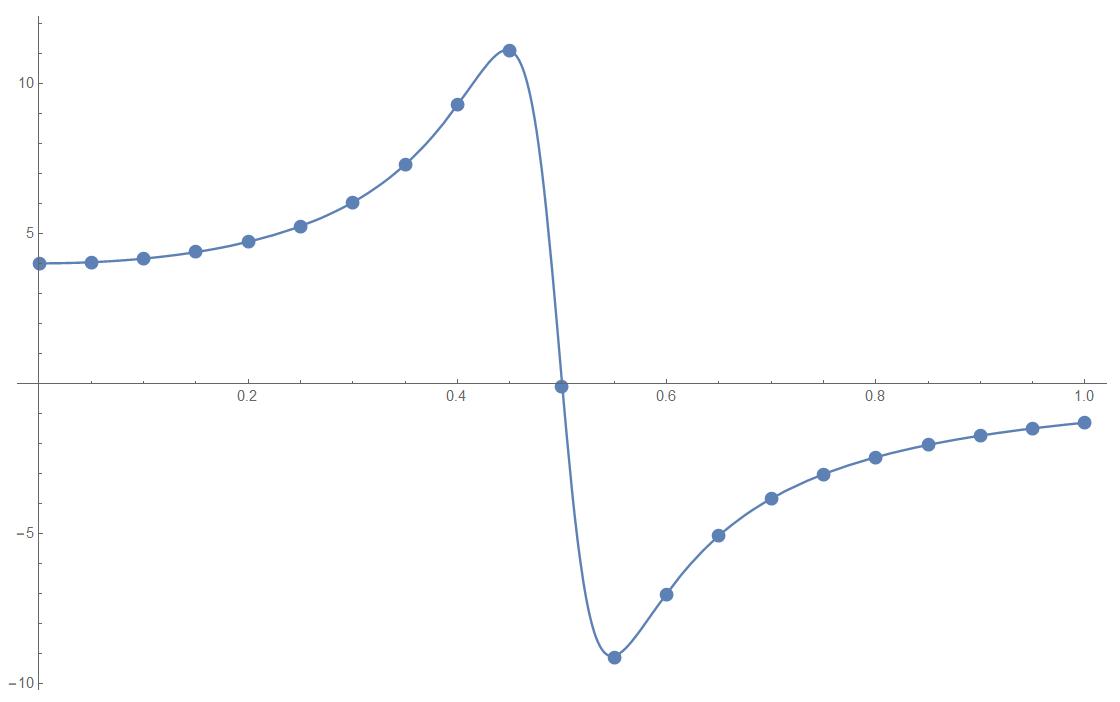
\includegraphics[width=\textwidth]{example-re-epsilon.PNG}
        \subcaption{$\Re \epsilon_\text{r}(\omega)$}
    \end{subfigure}
    \begin{subfigure}{0.45\textwidth}
        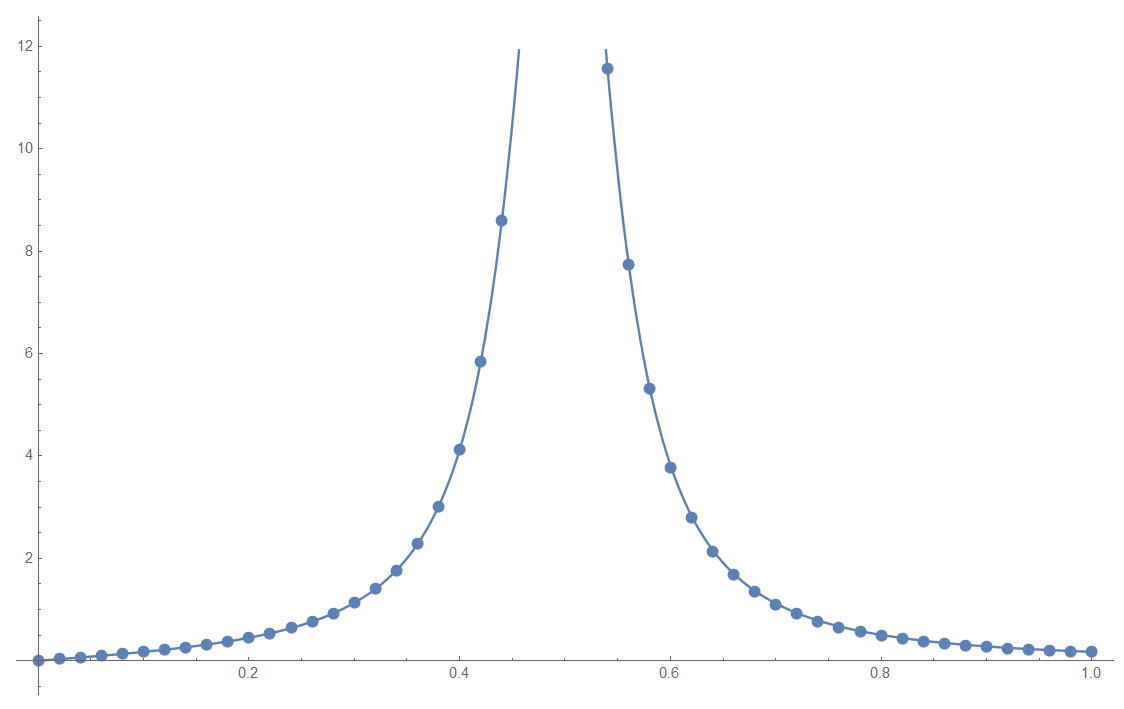
\includegraphics[width=\textwidth]{example-im-epsilon.PNG}
        \subcaption{$\Im \epsilon_\text{r}(\omega)$}
    \end{subfigure}
    \caption{Examples of figures obtained by \href{./homework-2-numerical-a.nb}{\texttt{homework-2-numerical-a.nb}}, where $\omega = 0.5, \gamma = 0.1$, and $L = 50, \epsilon = \num{1e-5}$. The points are obtained by numerically evaluating integrals on RHSs in \eqref{eq:kk-program}, and the curves are obtained by plotting the LHSs in \eqref{eq:kk-program}.}
    \label{fig:demo-curve}
\end{figure}

\begin{figure}
    \centering
    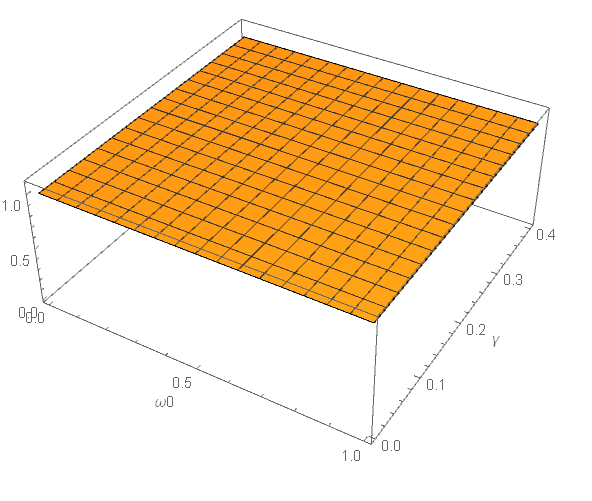
\includegraphics[width=0.6\textwidth]{sum-rule-im-epsilon.PNG}
    \caption{Numerical verification of \eqref{eq:im-epsilon-verify}, where we set $L=60$ and plot the LHS and it is found to always be unity. The code can be found in \href{./homework-2-numerical-c.nb}{\texttt{homework-2-numerical-c.nb}}.}
    \label{fig:im-epsilon-plot}
\end{figure}

\paragraph{}

\paragraph{Ground state with VW term in $G[n]$} Find the electron density and the electric potential of the ground state when the VW term is present in $G[n]$.

\paragraph{Solution} The electron density and the electric potential in the ground state are given by 
\begin{equation}
    \eval{\fdv{G}{n}}_0 + e \varphi_0 = \mu, \quad \laplacian \phi_0 = \frac{e}{\epsilon_0} (n_+ - n_0),
\end{equation}
where $e = - \abs*{e}$ is the charge carried by one electron, $\mu$ is the chemical potential, and the subscript 0 means the circumstance that $n = n_0$.
After introducing the VW term the energy functional is 
\begin{equation}
    G[n] = \int \dd[3]{\vb*{r}} g(n, \grad{n}), 
\end{equation}
where 
\begin{equation}
    g(n, \grad{n}) = \frac{3 \hbar^{2}}{10 m_{e}}\left(3 \pi^{2}\right)^{2 / 3} n^{5 / 3}+\frac{\lambda_{\mathrm{w}} \hbar^{2}}{8 m_{e}} \frac{\nabla n \cdot \nabla n}{n}+E_{\mathrm{xc}}.
\end{equation}

\end{document}